\capitulo{5}{Aspectos relevantes del desarrollo del proyecto}

En esta sección, se destacarán los elementos más significativos del desarrollo, proporcionando una perspectiva detallada de las decisiones adoptadas para alcanzar los objetivos del proyecto. Se resumirá la experiencia práctica, detallando cómo se abordaron los desafíos específicos, y se evaluará la importancia de estas soluciones en el contexto general del alcance del proyecto.

\section{Motivación del proyecto}

La motivación subyacente a este proyecto surge de la creciente importancia y demanda en el ámbito de la monitorización de invernaderos, especialmente en el contexto del cultivo de cannabis medicinal. La necesidad de implementar soluciones tecnológicas eficientes para garantizar condiciones óptimas de cultivo y maximizar la producción ha impulsado la elección de este tema.

El objetivo principal radica en diseñar un sistema económico y eficaz que permita a los cultivadores de cannabis medicinal supervisar las condiciones ambientales de sus invernaderos de manera remota. Este proyecto busca proporcionar una herramienta valiosa para mejorar la eficiencia, la calidad y la consistencia en la producción de cannabis medicinal, al tiempo que se abordan los desafíos específicos asociados con la monitorización de variables críticas como temperatura, humedad y luz.

\section{Formación necesaria}

El proyecto ha requerido una formación interdisciplinaria que abarca diversas áreas. En primer lugar, la comprensión profunda de los principios de la programación y el desarrollo de software ha sido esencial. La elección de la Raspberry Pi Pico W como plataforma y la programación en MicroPython para controlar los dispositivos hardware involucra un conocimiento sólido en programación embebida y desarrollo en entornos limitados.

Además, la utilización de sensores especializados, como el DHT22~\cite{manual:DHT22}, el BH1750~\cite{manual:BH1750} y el sensor de humedad del suelo~\cite{wiki:SensorHumedadSuelo}, ha demandado una comprensión detallada de los principios de operación de estos dispositivos y cómo integrar sus lecturas en el sistema general. Esto implica una formación técnica en electrónica y sensores.

La implementación de conceptos relacionados con el Internet de las cosas (IoT) y la comunicación inalámbrica mediante la Raspberry Pi Pico W~\cite{misc:RPiPicoW} también ha requerido conocimientos específicos en redes y protocolos de comunicación.

La integración de MQTT~\cite{MQTT} en el código MicroPython para la Raspberry Pi Pico W ha requerido conocimientos específicos sobre este protocolo de mensajería ligero diseñado para la eficiente comunicación entre dispositivos en redes IoT.

En resumen, la formación necesaria abarca habilidades en programación embebida, electrónica, redes, IoT y desarrollo de software. La combinación de estas competencias ha sido esencial para la ejecución exitosa del proyecto, demostrando la importancia de una formación integral y multidisciplinaria en el ámbito de la ingeniería y la tecnología.
\pagebreak

\section{Metodología}
Se ha optado por implementar el enfoque Scrum~\cite{misc:Scrum} como metodología principal para llevar a cabo el proyecto de manera iterativa y ágil. La intención fue recrear un entorno de trabajo lo más fiel posible a las dinámicas laborales, a pesar de las limitaciones de interacción con un equipo real. Se establecieron reglas generales mínimas:
\begin{itemize}
	\item Se estructuraron las tareas en sprints semanales.
	\item Después de cada sprint semanal, se entregó trabajo de manera incremental.
	\item En cada revisión de sprint, se planificaron las tareas para la siguiente semana.
	\item A través de revisiones semanales, el proyecto se mantuvo flexible, permitiendo la integración de cambios en trabajos pequeños y mejorando continuamente.
	\item La estimación de tiempos por tareas se llevó a cabo utilizando el método Kanban basado en la dificultad.
	\item El estado de los issues se gestionó a través de un Kanban, reflejando la evolución del trabajo.
\begin{itemize}

\begin{figure}[h]
    \centering
    
\includegraphics[width=0.6\textwidth]{img/herramientas/scrum.png}
    \caption{Logo de Scrum.} \label{Img:scrum}
\end{figure}

\section{Desarrollo del proyecto}

El propósito inicial radicaba en la recopilación de datos ambientales, tales como humedad, temperatura, intensidad de luz y humedad del suelo, con el fin de almacenarlos y presentarlos de manera gráfica.\\

%Más tarde, se implementó la funcionalidad de enviar alertas a través de Telegram~\cite{misc:Telegram} en caso de que los valores recopilados excedieran los umbrales ideales.
%Posteriormente, se llevó a cabo una revisión de los datos recopilados, abordando la limpieza y realizando un análisis estadístico para obtener perspectivas adicionales.

%Una vez definida la idea del TFG y los componentes hardware, surgía la interrogante: "¿Dónde enviar los datos? ¿Cómo gestionarlos?". La primera medida fue mostrar los datos en una pantalla OLED~\cite{manual:Oled} conectada a la protoboard. Sin embargo, al estar fuera de la red, surgieron nuevas incógnitas, ya que inicialmente se trató de un sistema unidireccional en el cual el sensor recolecta los datos y los muestra en la pantalla OLED.

%Frente a estos cuestionamientos, tomé la decisión de crear un servidor LAMP, que proporcionaría la solución a las preguntas planteadas.\\

%Basándome en esta información y en mi experiencia previa trabajando con "Smart Cities", tomo la decisión de enviar la información recopilada por los sensores al servidor mediante MQTT~\cite{manual:MQTT}. Esta elección permite la visualización en tiempo real de los datos en una página web alojada en el servidor LAMP cada vez que la placa junto con el sensor envíe datos. Además, posibilita el almacenamiento de los datos en la base de datos MySQL~\cite{misc:Mysql}, permitiéndome mantener un historial y realizar consultas.\\

%Listo, he leído e incluso almacenado los datos que se envían. Además, con la implementación de un bot de Telegram~\cite{misc:Telegram}, ahora puedo consultar en tiempo real la información proveniente de los sensores.\\
%\pagebreak

%\begin{figure}[h]
    %\centering
    %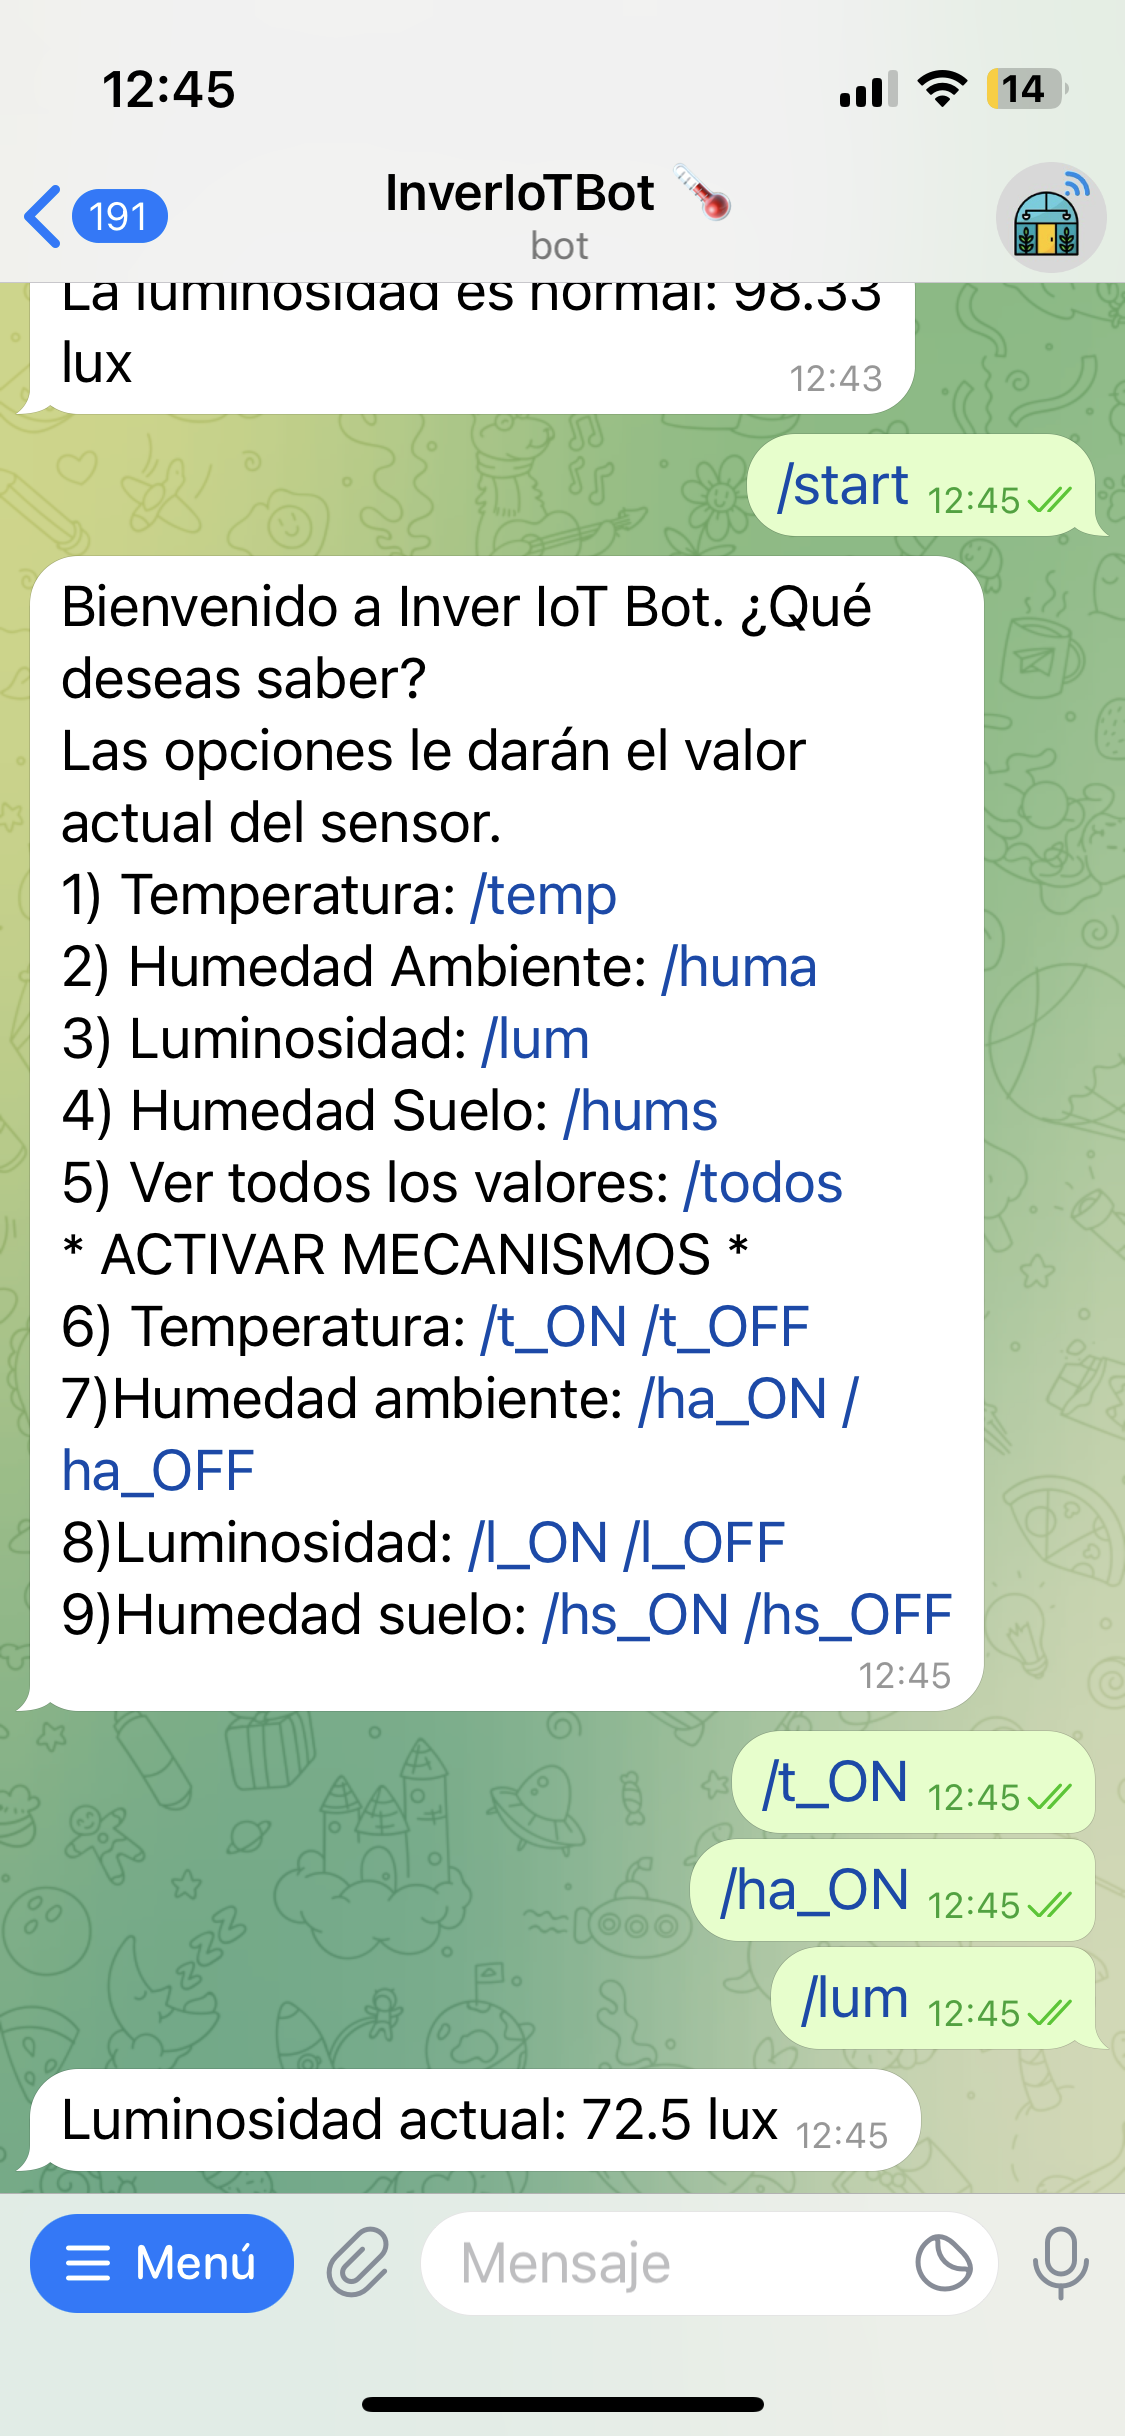
\includegraphics[width=0.6\textwidth]{img/desarrollo/BotTelegram_comandos.png}
    %\caption{Comandos del bot de Telegram.}
%\end{figure}

%También optamos por desarrollar una aplicación de escritorio para Windows en C\#~\cite{manual:C#}, que permite la visualización en tiempo real de los datos. ¡Problema resuelto! Ahora, puedo recibir y monitorear la temperatura, luminosidad y otros valores del invernadero. Sin embargo, al caer la noche, la luminosidad y la temperatura disminuyen, planteando un nuevo desafío. En este caso, necesitaría establecer una comunicación bidireccional con la placa Raspberry Pi Pico W para, por ejemplo, encender los focos y activar los calentadores.\\

%Este cambio a una comunicación bidireccional se logró suscribiendo la Raspberry Pi Pico W a un topic MQTT. Ahora, puedo enviar órdenes para procesarlas según sea necesario. Sin embargo, la activación de mecanismos físicos como encender focos, activar calefacción, regar el suelo o humidificar el ambiente aún no se ha implementado, ya que corresponde a otras especialidades como telecomunicación industrial o mecánica.\\

%El cannabis medicinal requiere condiciones ambientales constantes y dentro de un umbral específico para un crecimiento óptimo y delicado.\\

%Definimos umbrales (valor mínimo/máximo) para mantener los valores de los sensores dentro de límites aceptables. En caso de detectar un valor anómalo fuera de estos umbrales, se genera una alerta. Para esta función, empleamos un bot de Telegram que envía mensajes de alerta, y se configura un LED RGB para cada medición (temperatura, humedad, luminosidad, humedad del suelo). Si la temperatura es baja, por ejemplo, el LED se ilumina en azul y envía una alerta por Telegram; si la temperatura es alta, el LED se enciende en rojo. Un LED apagado indica valores normales dentro del umbral.\\

%La intervención manual también es posible, como activar ventiladores al observar un LED azul. Además, estos procesos pueden automatizarse. Por ejemplo, si la luminosidad cae por debajo del umbral, los focos se encienden hasta alcanzar el valor óptimo.\\

%La información se visualiza en tiempo real en una página web desarrollada con Node.js, incluyendo un histórico de datos almacenados en la base de datos. En este contexto, detallaré la configuración del servidor y la implementación de Node.js en la página web.\\ \\

\subsection{Hardware}
\begin{itemize}
	\item La Raspberry Pi Pico W estará situada en el invernadero para la recopilación de datos.
	\item Los LEDs RGB, instalados en la oficina del cliente, indicarán visualmente si los valores superan los umbrales establecidos.
	\item La pantalla OLED estará colocada en la puerta del invernadero para mostrar los valores actualizados.
\end{itemize}

\begin{figure}[h]
    \centering
    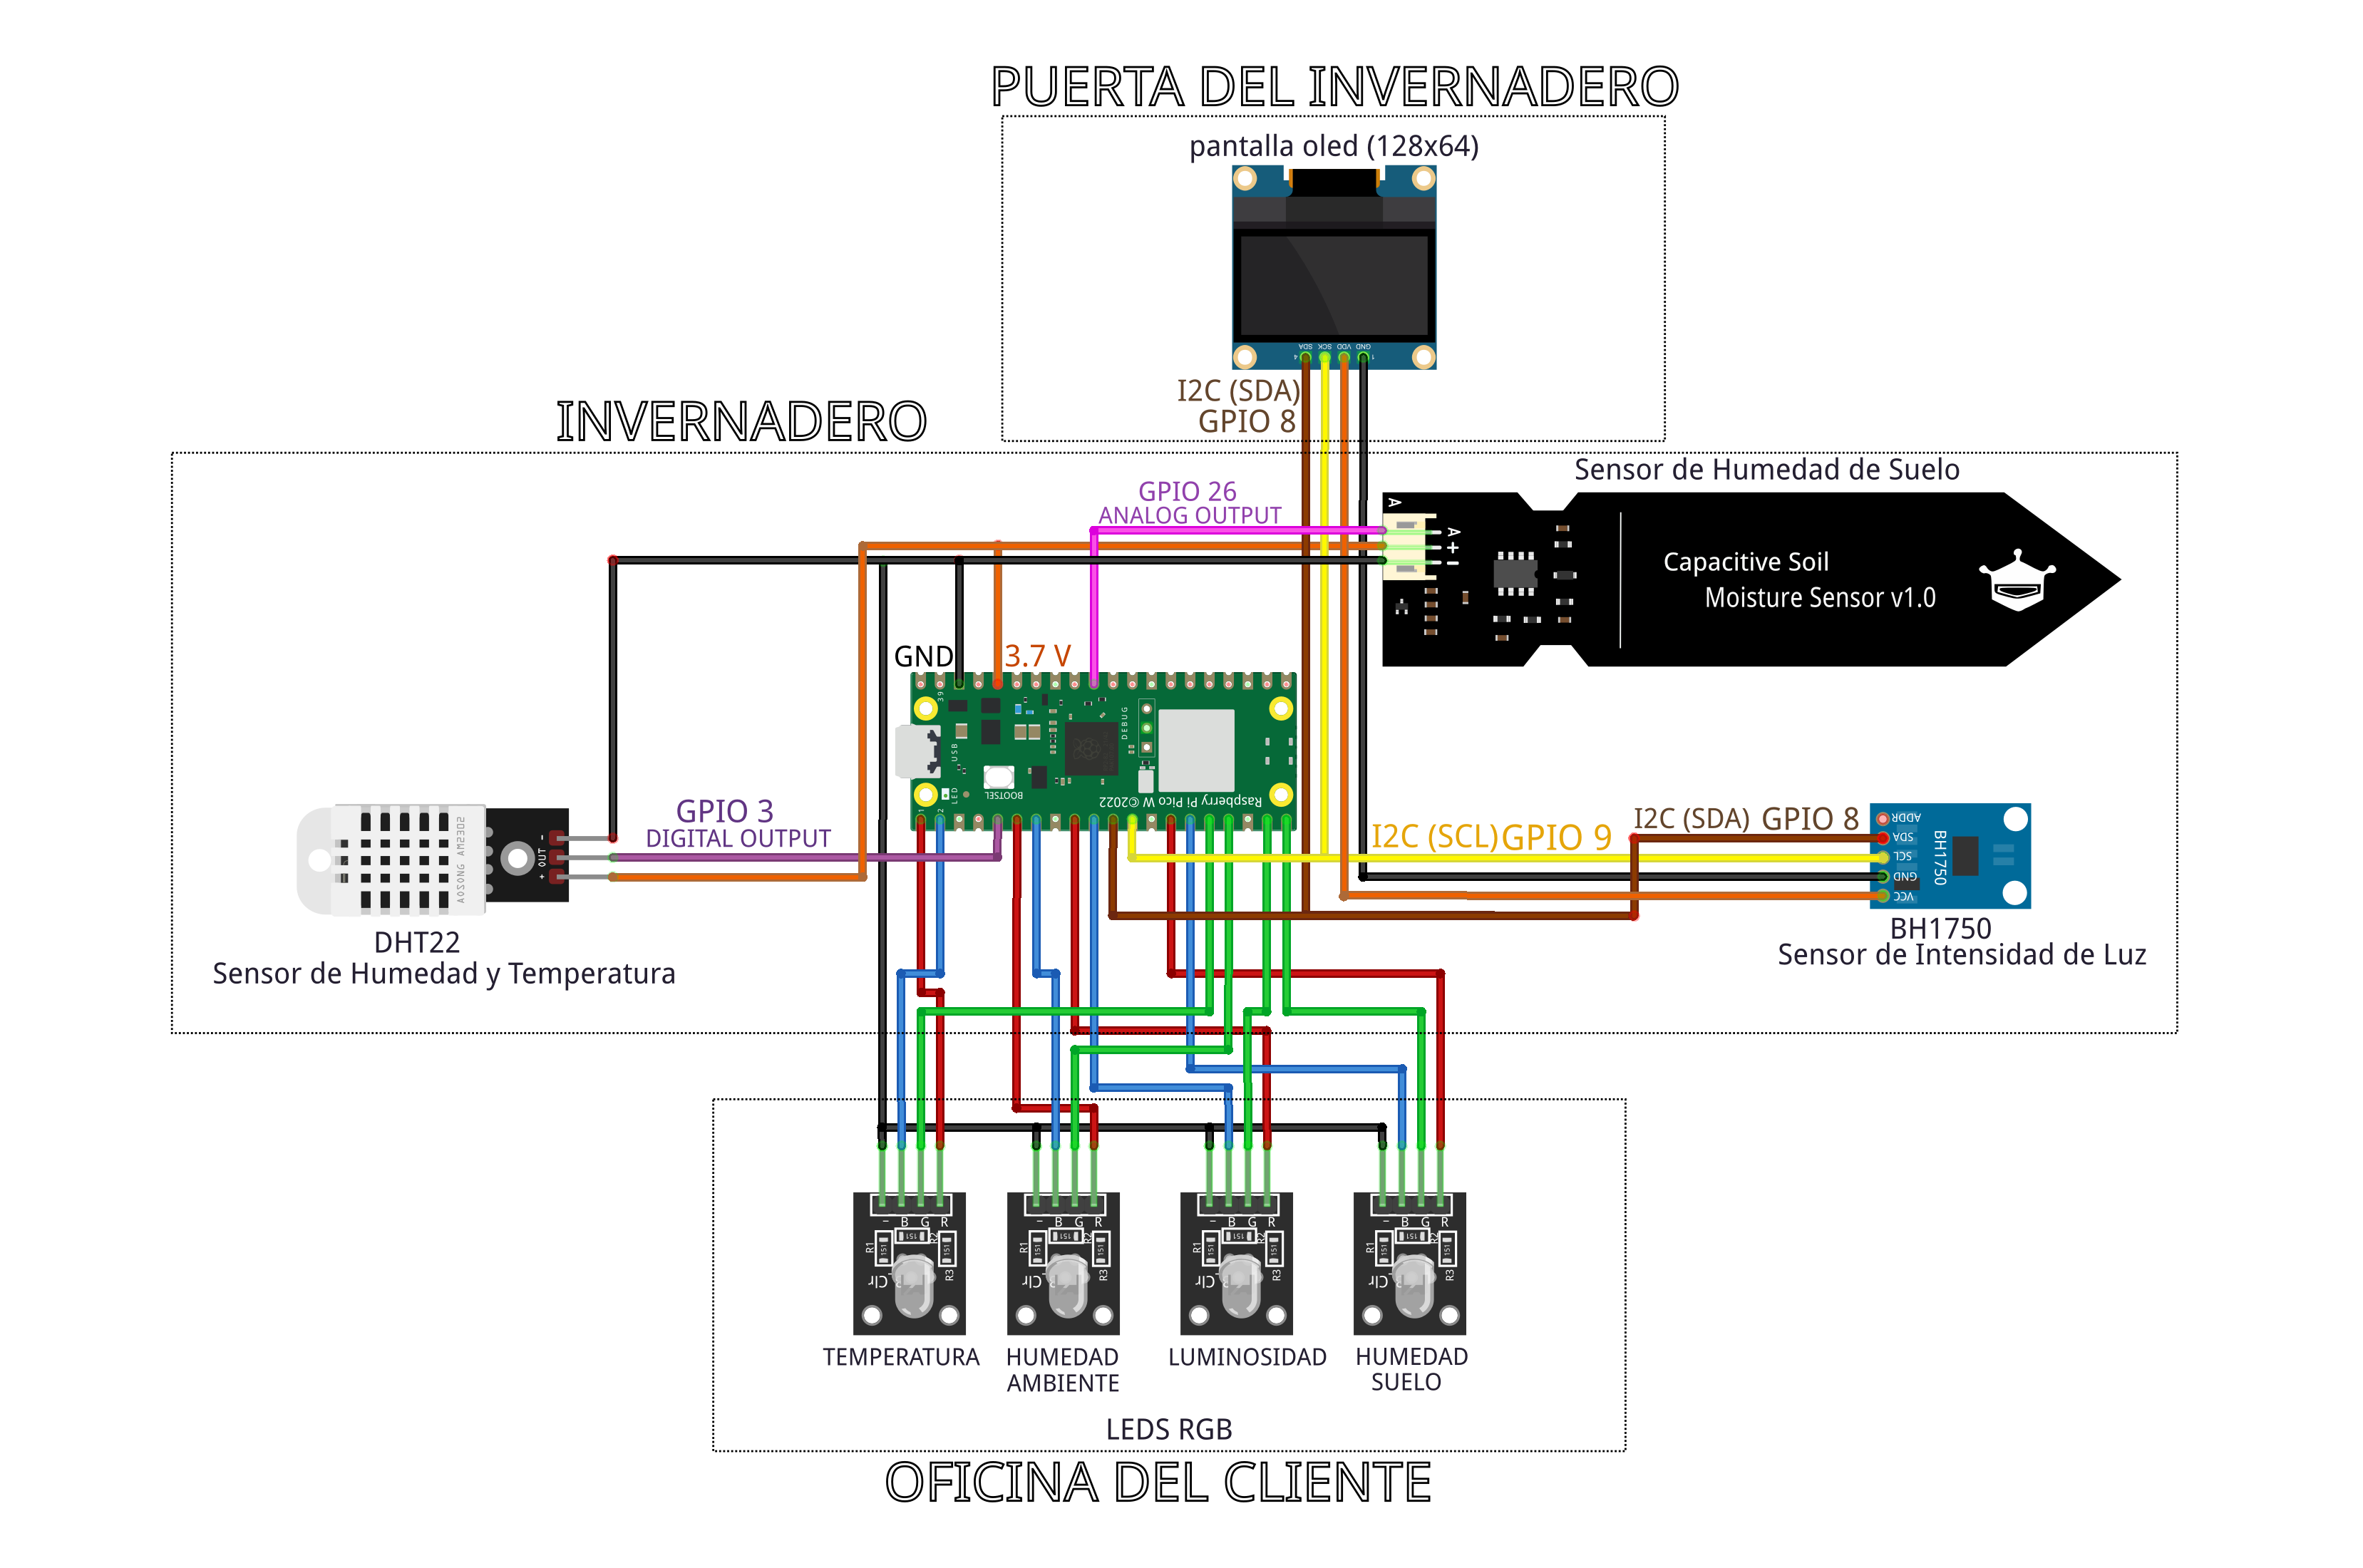
\includegraphics[width=0.8\textwidth]{img/diagramas/conexiones.png}
    \caption{Conexiones.} \label{Img:conexionesHardware}
\end{figure}
\pagebreak

\subsection{InverIoT}
Se desarrolla una aplicación de escritorio para Windows llamada InverIoT, que permite al usuario monitorizar en tiempo real los datos provenientes de los sensores conectados a la placa. Utilizando el protocolo MQTT~\cite{manual:MQTT}, la aplicación suscribe y recibe los datos publicados en el mismo tema. Estos datos son formateados y presentados en textboxes correspondientes, con unidades de medida agregadas. Se incorporan botones para activar o desactivar mecanismos, como un LED verde, que corrigen valores fuera de los umbrales ideales indicados en la parte derecha de la interfaz. Además, se añaden 8 textboxes en la parte inferior para ajustar manualmente los valores mínimos y máximos de cada parámetro. Los umbrales se actualizan desde la base de datos del servidor LAMP, proporcionando indicadores visuales de color azul para valores bajos, gris para valores normales y rojo para valores altos.

Se desarrolló la aplicación de escritorio utilizando Windows Forms y programada en lenguaje \textbf{C\#}~\cite{manual:C#}.

\begin{figure}[h]
    \centering
    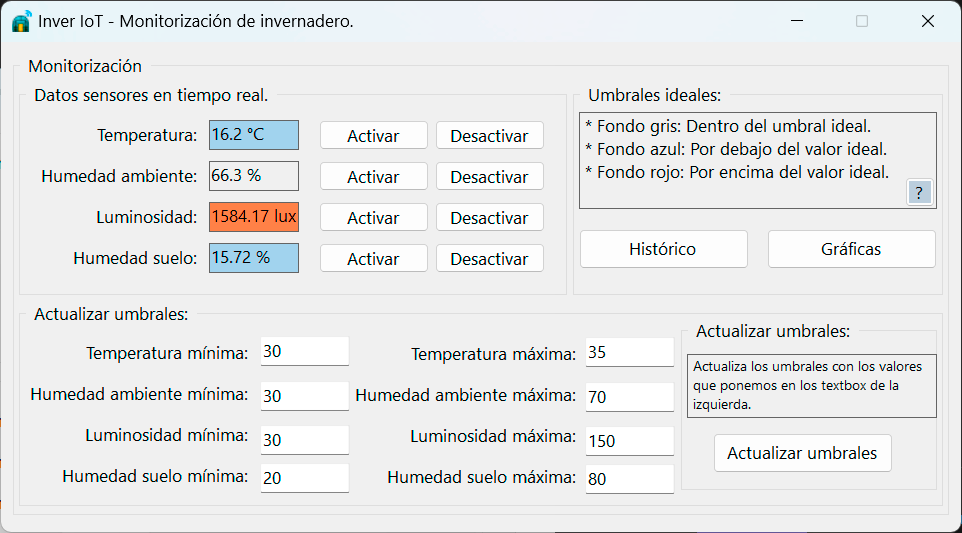
\includegraphics[width=1\textwidth]{img/desarrollo/InverIoT_Desktop.png}
	\caption{Aplicación de escritorio \textbf{InverIoT}.}
\end{figure}
\pagebreak

\begin{figure}[h]
    \centering
    \includegraphics[width=0.9\textwidth]{img/desarrollo/InverIoT_Histórico.png}
    \caption{Historial de los datos.}
\end{figure}


\begin{figure}[h]
    \centering
    \includegraphics[width=0.9\textwidth]{img/desarrollo/InverIoT_Gráficas.png}
    \caption{Gráfica mostrando los datos en un intervalo de fechas.}
\end{figure}
\pagebreak

\subsection{Dashboard}
Se desarrolla un dashboard que permite al usuario visualizar en tiempo real los datos capturados por los sensores, con una interfaz similar a la aplicación de escritorio. Los valores que exceden los umbrales establecidos se destacan mediante cambios de color. La plataforma incluye una gráfica en tiempo real y la capacidad de acceder a un historial con filtro de fecha. Los umbrales utilizados se extraen de la tabla \textbf{TFG\_UBU} en la base de datos MySQL~\cite{misc:Mysql}.

El panel de control está disponible para su acceso a través del siguiente enlace: \href{http://www.inveriot.com}{InverIoT Dashboard}

\begin{figure}[h]
    \centering
    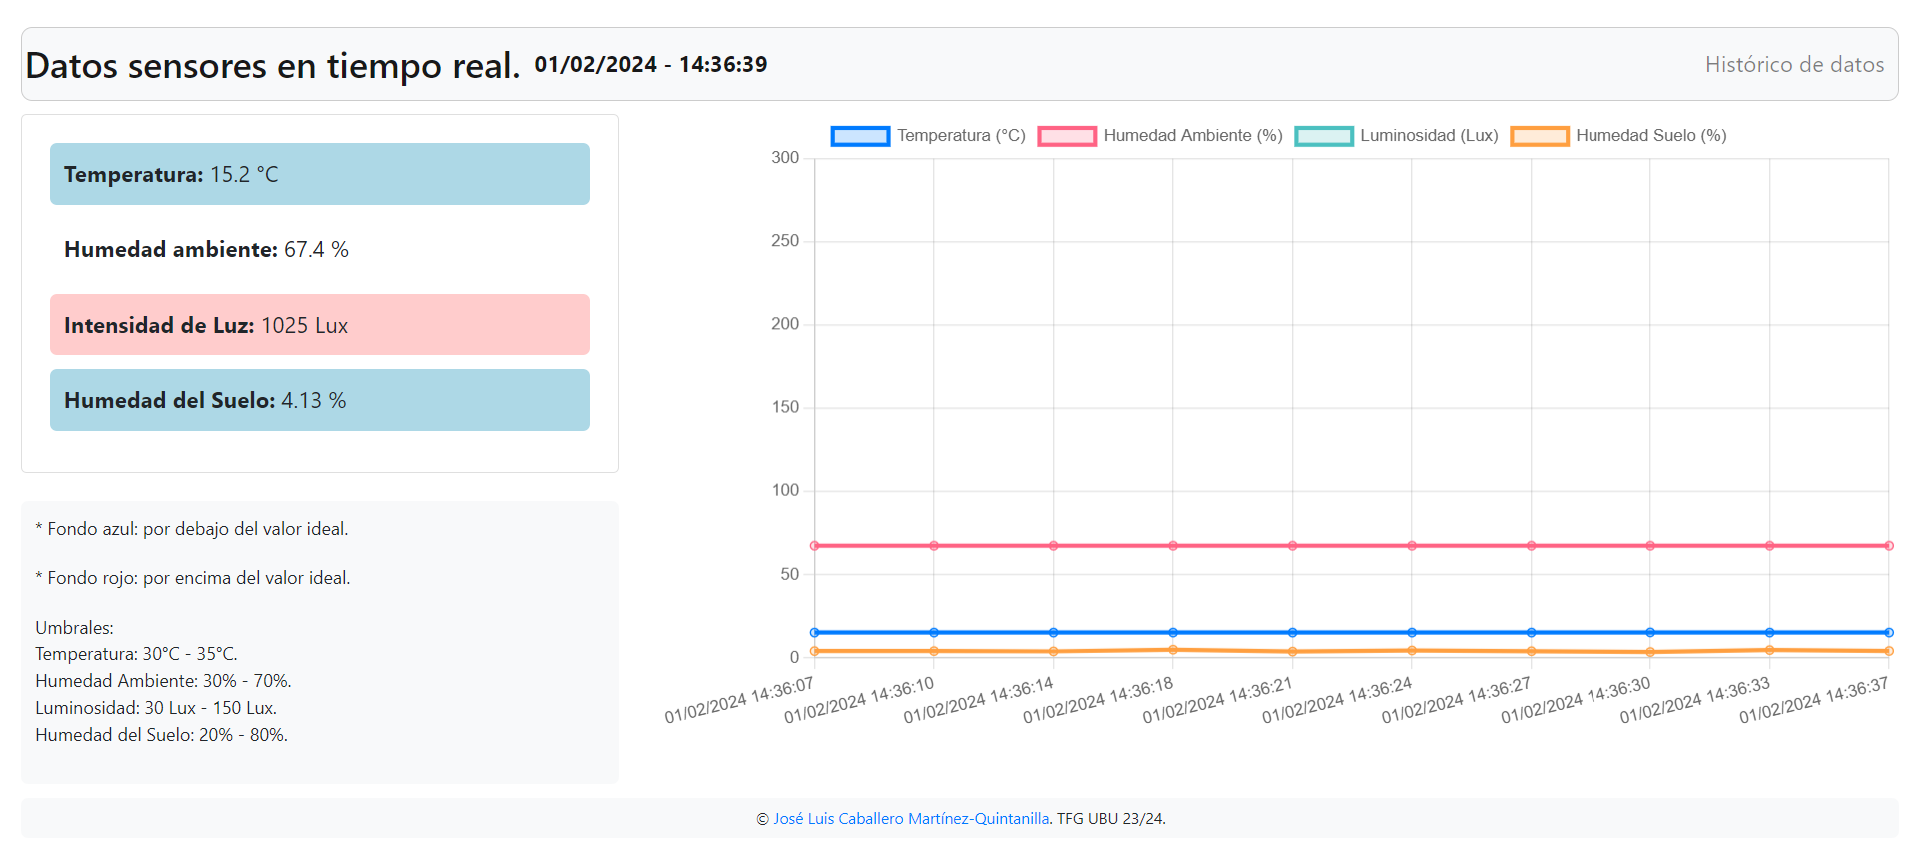
\includegraphics[width=0.8\textwidth]{img/desarrollo/Dashboard1.png}
    \caption{Intensidad de luz superando los umbrales.} \label{Img:Dashboard1}
\end{figure}

\begin{figure}[h]
    \centering
    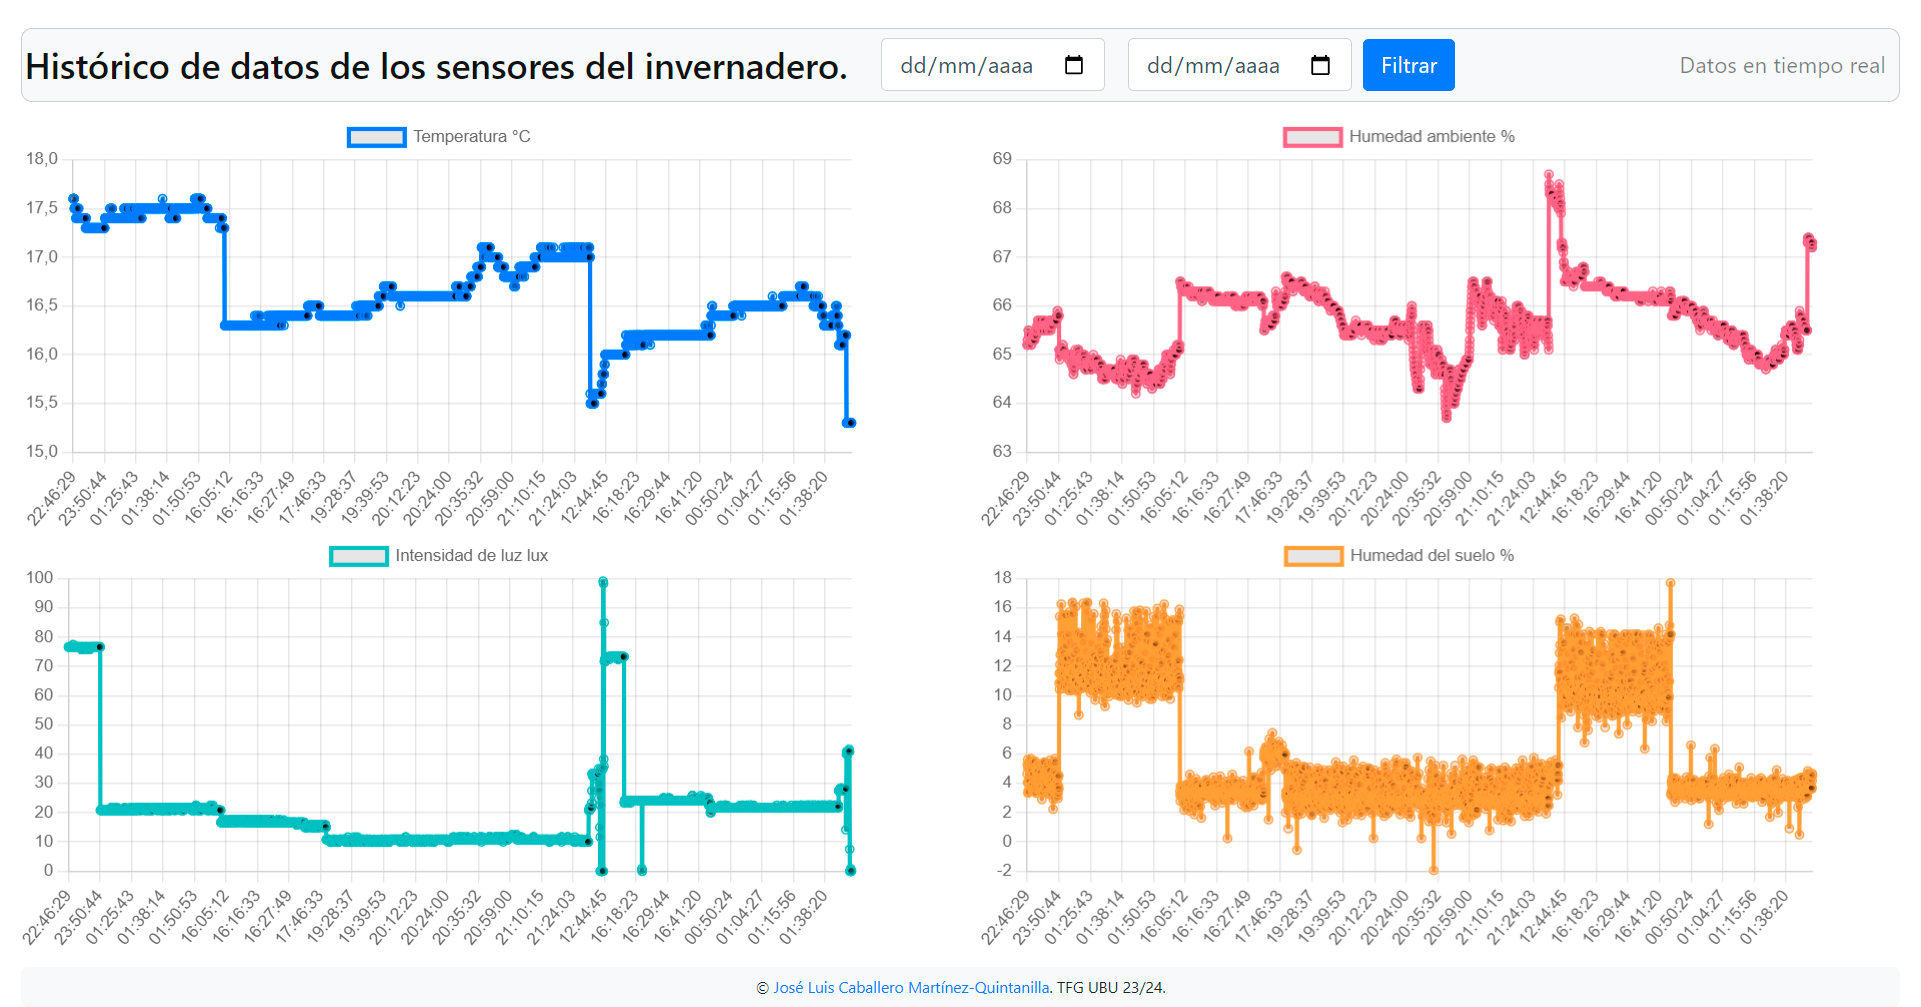
\includegraphics[width=0.8\textwidth]{img/desarrollo/Dashboard_Historico.png}
    \caption{Vista del historial: al cargar, muestra los datos del día actual.} \label{Img:Dashboard_Historico}
\end{figure}

\subsection{NodeMqtt}
\textbf{nodeMqtt} es un servicio en Node.js~\cite{misc:Nodejs} que escucha los topics \textbf{invernadero/sensores} e \textbf{invernadero/umbrales}. Los datos son enviados por la placa Raspberry Pi Pico W RP2040~\cite{misc:RPiPicoW}, que recopila valores de sensores. El servicio \textbf{nodeMqtt} captura, formatea y luego inserta estos datos en la base de datos MySQL~\cite{misc:Mysql} para los valores de sensores, además de actualizar los umbrales correspondientes.

Está conformado por los siguientes archivos:
\begin{itemize}
	\item \textbf{index.js:}
		Es el punto de entrada del código de la aplicación.
	\item \textbf{package.json:}
		Es un archivo de configuración que describe la aplicación y sus dependencias.
\end{itemize}

%Este apartado pretende recoger los aspectos más interesantes del desarrollo del proyecto, comentados por los autores del mismo.
%Debe incluir desde la exposición del ciclo de vida utilizado, hasta los detalles de mayor relevancia de las fases de análisis, diseño e implementación.
%Se busca que no sea una mera operación de copiar y pegar diagramas y extractos del código fuente, sino que realmente se justifiquen los caminos de solución que se han tomado, especialmente aquellos que no sean triviales.
%Puede ser el lugar más adecuado para documentar los aspectos más interesantes del diseño y de la implementación, con un mayor hincapié en aspectos tales como el tipo de arquitectura elegido, los índices de las tablas de la base de datos, normalización y desnormalización, distribución en ficheros3, reglas de negocio dentro de las bases de datos (EDVHV GH GDWRV DFWLYDV), aspectos de desarrollo relacionados con el WWW...
%Este apartado, debe convertirse en el resumen de la experiencia práctica del proyecto, y por sí mismo justifica que la memoria se convierta en un documento útil, fuente de referencia para los autores, los tutores y futuros alumnos.
